\documentclass[a4paper,12pt]{report}
\usepackage{mathtext}
\usepackage[T2A]{fontenc}
\usepackage[utf8]{inputenc}
\usepackage[english,russian]{babel}
\usepackage{geometry}
\usepackage{listings}
\usepackage{amsmath}
\geometry{top=2cm}
\usepackage{titlesec}
\usepackage{color}
\usepackage{pgfplots}
\usepackage{filecontents}
\usetikzlibrary{datavisualization}
\usetikzlibrary{datavisualization.formats.functions}
\usepackage{caption}
\DeclareCaptionFont{white}{\color{white}}
\DeclareCaptionFormat{listing}{\colorbox{gray}{\parbox{\textwidth}{#1#2#3}}}
\captionsetup[lstlisting]{format=listing,labelfont=white,textfont=white}

% Для листинга кода:
\lstset{ %
language=C++,                 % выбор языка для подсветки
basicstyle=\small\sffamily, % размер и начертание шрифта для подсветки кода
numbers=left,               % где поставить нумерацию строк (слева\справа)
numberstyle=\tiny,           % размер шрифта для номеров строк
stepnumber=1,                   % размер шага между двумя номерами строк
numbersep=-5pt,                % как далеко отстоят номера строк от подсвечиваемого кода
showspaces=false,
backgroundcolor=\color{white},         
showstringspaces=false,      % показывать или нет пробелы в строках
showtabs=false,             % показывать или нет табуляцию в строках
frame=single,              % рисовать рамку вокруг кода
tabsize=2,                 % размер табуляции по умолчанию равен 2 пробелам
captionpos=t,              % позиция заголовка вверху [t] или внизу [b] 
breaklines=true,           % автоматически переносить строки (да\нет)
breakatwhitespace=false, % переносить строки только если есть пробел
escapeinside={\%*}{*)},   % если нужно добавить комментарии в коде
	    keywordstyle=\color{blue}\ttfamily,
	    stringstyle=\color{red}\ttfamily,
	    commentstyle=\color{green}\ttfamily,
	    morecomment=[l][\color{magenta}]{\#},
	    columns=fullflexible   % если нужно добавить комментарии в коде
}

% Для измененных титулов глав:
\definecolor{gray75}{gray}{0.75} % определяем цвет
\newcommand{\hsp}{\hspace{20pt}} % длина линии в 20pt
% titleformat определяет стиль
\titleformat{\chapter}[hang]{\Huge\bfseries}{\thechapter\hsp\textcolor{gray75}{|}\hsp}{0pt}{\Huge\bfseries}


\begin{document}
\begin{titlepage}
	\centering
	{\scshape\LARGE МГТУ им. Н.Э.Баумана \par}
	\vspace{4cm}
	{\scshape\Large Лабораторная работа №5\par}
	\vspace{0.5cm}	
	{\scshape\Large По курсу: "Анализ алгоритмов"\par}
	\vspace{2cm}
	{\huge\bfseries Конвейерная обработка данных \par}
	\vspace{3cm}
	\Large Работу выполнил: Луговой Дмитрий, ИУ7-51Б\par
	\vspace{0.5cm}
	\Large Преподаватель:  Волкова Л.Л.\par

	\vfill
	\large \textit {Москва, 2019} \par
\end{titlepage}

\setcounter{page}{2}

\tableofcontents

\newpage
\chapter*{Введение}
\addcontentsline{toc}{chapter}{Введение}
\hspace{0.6cm}  \textbf{Конвейер} — способ организации вычислений, используемый в современных процессорах и контроллерах с целью повышения их производительности (увеличения числа инструкций, выполняемых в единицу времени — эксплуатация параллелизма на уровне инструкций), технология, используемая при разработке компьютеров и других цифровых электронных устройств.

\textbf{Цель работы}: Получить навык организации асинхронной передачи данных между потоками на примере конвейерной обработки информации.\\\\

\textbf{\LARGE Задачи работы}\\\\
Задачами данной лабораторной являются:
\begin{enumerate}
\item[1)] Выбрать и описать методы обработки данных, которые будут сопоставлены методам конвейера;
\item[2)] Описать архитектуру программы, а именно какие функции имеет главный поток, принципы и алгоритмы обмена данными между потоками;
\item[3)] Реализовать конвейерную систему, а также сформировать лог событий с указанием времени их происхождения, описать реализацию;
\item[4)] Интерпретировать сформированный лог.
\end{enumerate}


\chapter{Аналитическая часть}
\hspace{0.6cm}В данном разделе содержится описание работы конвейера.

\section{Идея конвееризации}
\hspace{0.6cm}Конвейеризация (или конвейерная обработка) в общем случае основана на разделении подлежащей исполнению функции на более мелкие части, называемые ступенями, и выделении для каждой из них отдельного блока аппаратуры. Производительность при этом возрастает благодаря тому, что одновременно на различных ступенях конвейера выполняются несколько команд.

Идея заключается в параллельном выполнении нескольких инструкций процессора. Сложные инструкции процессора представляются в виде последовательности более простых стадий. Вместо выполнения инструкций последовательно (ожидания завершения конца одной инструкции и перехода к следующей), следующая инструкция может выполняться через несколько стадий выполнения первой инструкции. Это позволяет управляющим цепям процессора получать инструкции со скоростью самой медленной стадии обработки, однако при этом намного быстрее, чем при выполнении эксклюзивной полной обработки каждой инструкции от начала до конца.

Выполнение каждой команды складывается из ряда последовательных этапов (шагов стадий), суть которых не меняется от команды к команде. С целью увеличения быстродействия процессора и максимального использования всех его возможностей в современных микропроцессорах используется конвейерный принцип обработки информации. Этот принцип подразумевает, что в каждый момент времени процессор работает над различными стадиями выполнения нескольких команд, причем на выполнение каждой стадии выделяются отдельные аппаратные ресурсы. По очередному тактовому импульсу каждая команда в конвейере продвигается на следующую стадию обработки, выполненная команда покидает конвейер, а новая поступает в него

\section{Задача конвееризации}

\hspace{0.6cm}Конвейер будет состоять из трех уровней. Генератор подает на вход конвейера (первый уровень) некоторые числа. Далее на каждом уровне осуществляется обработка данных, занимающая определенное время. Обработанные данные передаются последовательно с одного уровня (одной ленты) конвейера на следующий (следующую ленту). Для организации работы каждой ленты будет использована очередь задач, которые должны обработаться на этой ленте. Таким образом, лента будет работать, пока в её очереди есть задачи, но задачи попадают в очередь только в том случае, если данные уже были обработаны на предыдущем уровне или если их только сформировал генератор (для первой ленты). При этом время обработки на какой-либо ленте не должно сильно отличаться от времени обработки на остальных лентах, так как в противном случае возможны ситуации простоя одной или нескольких лент конвейера. На последнем уровне конвейера обработанные объекты попадают в результирующий пул. После завершения работы конвейера, то есть после завершения работы третьей ленты, проверяется равенство количества поданных на вход конвейера объектов количеству объектов в результирующем пуле. Если равенство верное, то конвейер отработал корректно, иначе где-то произошла ошибка и какие-то данные были обработаны неправильно, либо вообще были потеряны.

На каждом уровне конвейера алгоритм обработки информации заменяется задержкой выполняемой программы по времени для создания видимости работы ленты.

\section{Вывод}
\hspace{0.6cm}Таким образом, конвейеризация алгоритмов, на вход которых поступают однообразные данные, позволяет ускорить процесс обработки этих данных.

\chapter{Конструкторская часть}
\hspace{0.6cm}В этом разделе содержится описание реализации работы конвейера, cхемы работы конвейера и его лент.

\section{Описание реализации конвеера}

\hspace{0.6cm}Каждой ленте конвейера выделен отдельный поток. В главном потоке  запускаются все три рабочих потока - ленты конвейера. Для каждого потока есть своя очередь, в которой содержатся индекс выполняемой задачи и время в миллисекундах, необходимое на выполнение задачи (время задержки). Также в главном потоке генерируются входные данные, которые помещаются в очередь для первого потока. После завершения работы всех рабочих потоков проверяется список результирующих элементов и выводится сообщение о результате работы конвейера. В рабочих потоках извлекается очередной элемент из соответствующей очереди, вносится запись в лог-файл о начале обработки очередного элемента, выполняется задержка по времени. После этого новое значение помещается в очередь для следующего потока (или в список обработанных значений если обработка происходит уже в третьем потоке) и далее в лог-файл заносится запись о завершении обработки очередного элемента на определенной ленте (в определенном потоке). После окончания работы генератора в первую очередь записывается значение “-1”, что говорит о завершении работы конвейера. Это значение передается из очереди в очередь по лентам. На Рис. 2.1 представлена общая схема работы конвейера.

\begin{figure}[ht!]
\center{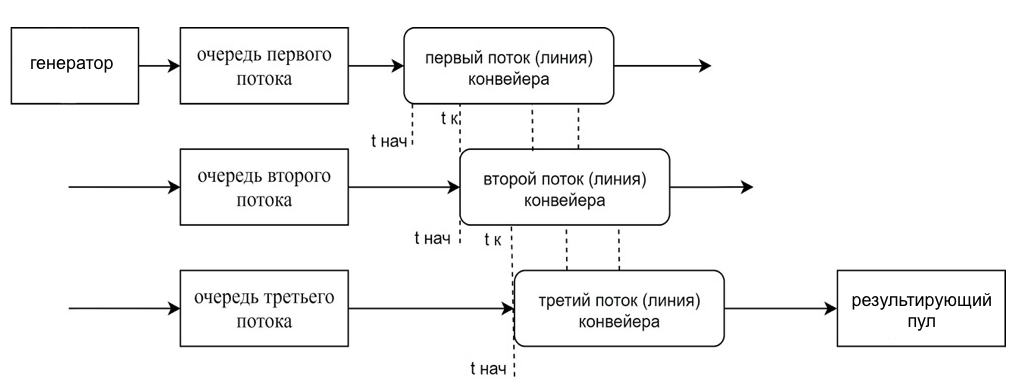
\includegraphics[scale=0.45]{Conveyor.png}}
\caption{Схема работы конвеера}
\end{figure}

\newpage

На рисунках 2.2 - 2.3 будет представлены схемы алгоритмов работы основного потока и первой ленты (остальные ленты реализованы аналогично).

\begin{figure}[ht!]
\center{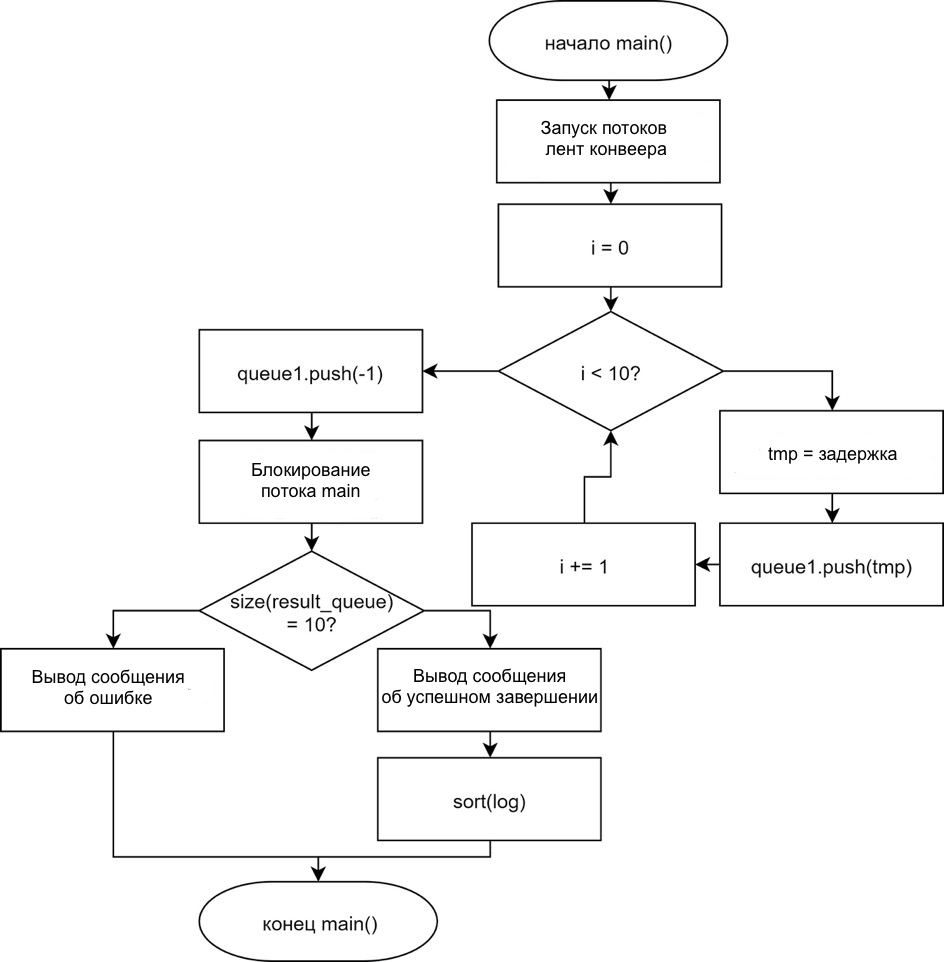
\includegraphics[scale=0.5]{MainThread.png}}
\caption{Схема работы основного потока}
\end{figure}

\newpage

\begin{figure}[ht!]
\center{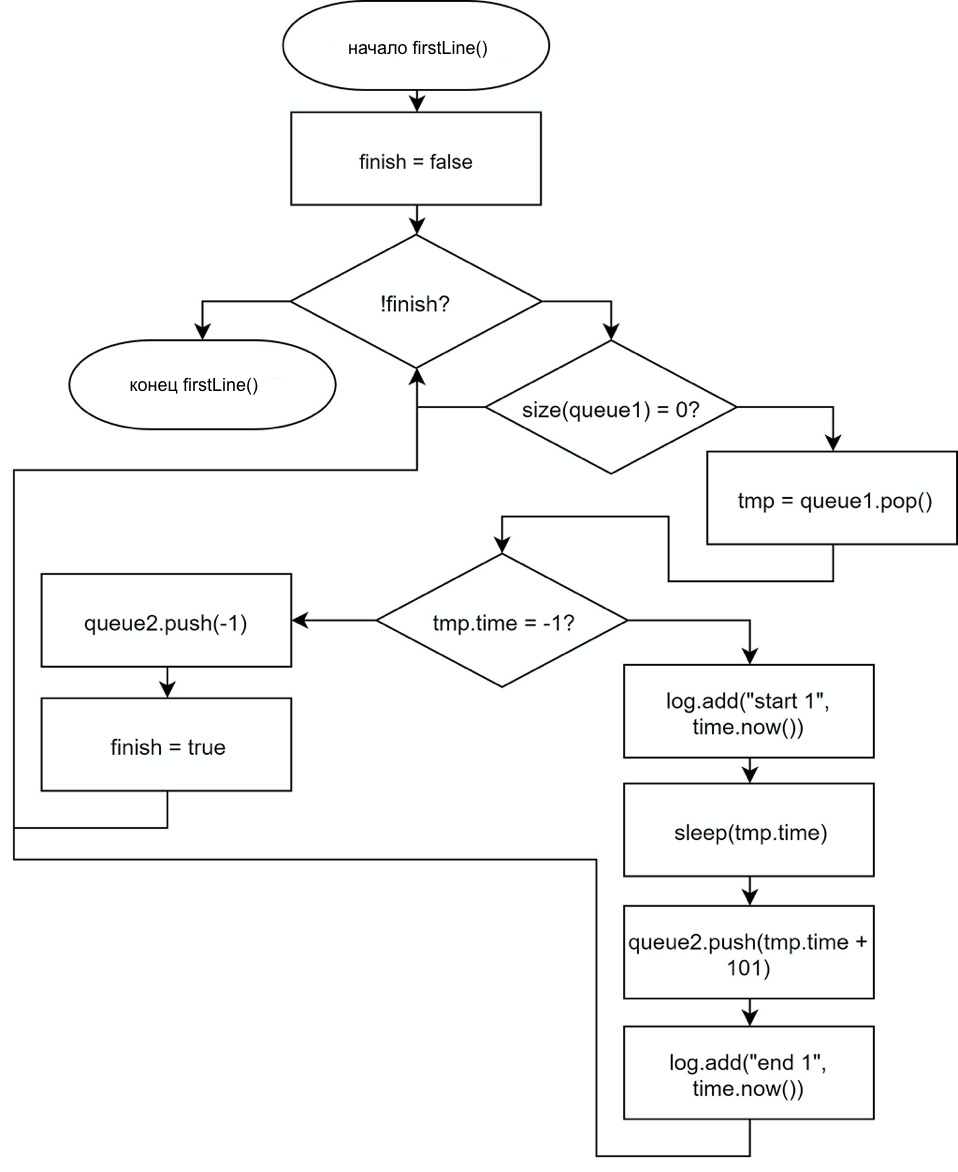
\includegraphics[scale=0.5]{fistLine.png}}
\caption{Схема работы первой ленты}
\end{figure}

\section{Вывод}
Была разработаны структура алгоритма, использующего конвейерную обработку данных.

\chapter{Технологическая часть}
\hspace{0.6cm}В данном разделе приведены требования к программному обеспечению, средства реализации и листинги кода
\section{Требования к ПО}

\hspace{0.6cm}На вход поступает значение задержки при обработке данных на линиях.
	
\section{Средства реализации}
\hspace{0.6cm}Для реализации представленных алгоритмов был выбран язык C++. Время работы алгоритмов было замерено с помощью функции system\_clock() из библиотеки chrono. Для тестирования использовался компьютер на базе процессора Intel Core i5 (4 физических ядра, 8 логических).

\section{Листинги кода}

\hspace{0.6cm}В Листинге 3.1 показана реализация главного потока.

\begin{lstlisting}[caption=Функция главного потока]
  int main()
  {
      thread lineOne(&firstLine);
      thread lineTwo(&secondLine);
      thread lineThree(&thirdLine);
      for(int i = 0; i < nItems; ++i)
      {
          int inTime = 1000;
          cout << "Item: " << i << ", value: " << inTime << " was added." << endl;
          inMtx.lock();
        i  nQue.push({i, inTime});
        i  nMtx.unlock();
          std::this_thread::sleep_for(std::chrono::milliseconds(50));
      }
      inMtx.lock();
      inQue.push({-1, -1});
      inMtx.unlock();
  
      lineOne.join();
      lineTwo.join();
      lineThree.join();
      if (outQue.size() == nItems)
      {
          cout << "Conveyor finished his work successfully." << endl;
          sortLog();
          createLog("log.txt");
          cout << "Conveyor took: " << logMessages[logMessages.size() - 1].first - logMessages[0].first << " seconds." << endl;
      }
      else
      {
          cout << "Conveyor missed " << nItems - outQue.size() << " items.\n"<< endl;
      }
      return 0;
  }
\end{lstlisting}

В Листингах 3.2, 3.3, 3.4 показаны реализации функций для линий конвейера.

\begin{lstlisting}[caption=Функция первой линии конвеера]
  void firstLine()
  {
      bool finish = false;
      while (!finish)
      {
          inMtx.lock();
          if (!inQue.empty())
          {
              pair<int, int> curItem = inQue.front();
              inQue.pop();
              int index = curItem.first;
              int t0 = curItem.second;
              if (index != -1)
              {
                  logMtx1.lock();
                  string tmp = "Line 1: Starting processing item " + to_string(index) + ", value: " + to_string(t0) + " milliseconds";
                  logMessages.push_back({currentTime(), tmp});
                  logMtx1.unlock();
                  std::this_thread::sleep_for(std::chrono::milliseconds(t0));
                  tmpMtx1.lock();
                  tmpQue1.push({index, t0});
                  tmpMtx1.unlock();

                  logMtx1.lock();
                  tmp = "Line 1: Finished processing item " + to_string(index);
                  logMessages.push_back({currentTime(), tmp});
                  logMtx1.unlock();
              }
              else
              {
                  tmpMtx1.lock();
                  tmpQue1.push({-1, -1});
                  tmpMtx1.unlock();
                  finish = true;
              }
          }
          inMtx.unlock();
      }
  }
\end{lstlisting}

\begin{lstlisting}[caption=Функция  второй линии конвеера]
void secondLine()
  {
      bool finish = false;
      while(!finish)
      {
          tmpMtx1.lock();
          if (!tmpQue1.empty())
          {
              pair<int, int> curItem = tmpQue1.front();
              int index = curItem.first;
              int t0 = curItem.second;
              tmpQue1.pop();
              if (t0 != -1)
              {
                  logMtx1.lock();
                  string tmp = "Line 2: Starting processing item " + to_string(index) + ", value: " + to_string(t0) + " milliseconds";
                  logMessages.push_back({currentTime(), tmp});
                  logMtx1.unlock();

                  std::this_thread::sleep_for(std::chrono::milliseconds(t0));
  
                  tmpMtx2.lock();
                  tmpQue2.push({index, t0});
                  tmpMtx2.unlock();

                  logMtx1.lock();
                  tmp = "Line 2: Finished processing item " + to_string(index);
                  logMessages.push_back({currentTime(), tmp});
                  logMtx1.unlock();
              }
              else
              {
                  tmpMtx2.lock();
                  tmpQue2.push({-1, -1});
                  tmpMtx2.unlock();
                  finish = true;
              }
          }
          tmpMtx1.unlock();
      }
  }
\end{lstlisting}

\begin{lstlisting}[caption=Функция третьей линии конвеера]
    void thirdLine()
    {
        bool finish = false;
        while(!finish)
        {
            tmpMtx2.lock();
            if (!tmpQue2.empty())
            {
                pair<int, int> curItem = tmpQue2.front();
                int index = curItem.first;
                int t0 = curItem.second;
                tmpQue2.pop();
                if (t0 != -1)
                {
                    logMtx1.lock();
                    string tmp = "Line 3: Starting " + to_string(index) + " item, value: " + to_string(t0) + " milliseconds";
                    logMessages.push_back({currentTime(), tmp});
                    logMtx1.unlock();
                    std::this_thread::sleep_for(std::chrono::milliseconds(t0));
                    outMtx.lock();
                    outQue.push({index, t0});
                    outMtx.unlock();
                    logMtx1.lock();
                    tmp = "Line 3: Finished processing item " + to_string(index);
                    logMessages.push_back({currentTime(), tmp});
                    logMtx1.unlock();
                }
                else
                {
                    finish = true;
                }
            }
            tmpMtx2.unlock();
        }
    }
\end{lstlisting}

В Листинге 3.5 показана реализация функции сортировки лога.

\begin{lstlisting}[caption=Функция сортировки лога]
    void sortLog()
    {
        bool flag;
        for (size_t i = 0; i < logMessages.size(); i++)
        {
            flag = false;
            for (size_t j = 1; j < logMessages.size() - i; j ++)
            {
                if (logMessages[j].first < logMessages[j - 1].first)
                {
                    pair<time_t, string> tmp = logMessages[j];
                    logMessages[j] = logMessages[j - 1];
                    logMessages[j - 1] = tmp;
                    flag = true;
                }
            }
            if (!flag) return;
        }
    }
\end{lstlisting}

\section{Вывод}
Была реализован алгоритм, использующий конвейерную обработку данных, и осуществлена запись результатов в лог.

\chapter{Экспериментальная часть}
\hspace{0.6cm}В данном разделе будут приведены примеры работы программы, а также будет приведена интерпретация сформированного программой лог-файла.
\section{Примеры работы}
\hspace{0.6cm}На рисунках 4.1 - 4.3 приведены примеры работы программы. В консоль выводятся входные данные (данные для первой ленты конвейера) и результат прохождения этих данных через конвейер.
\begin{figure}[ht!]
\center{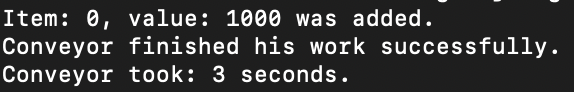
\includegraphics[scale=1]{Element1.png}}
\caption{Результат работы при 1 входном элементе}
\end{figure}

\begin{figure}[ht!]
\center{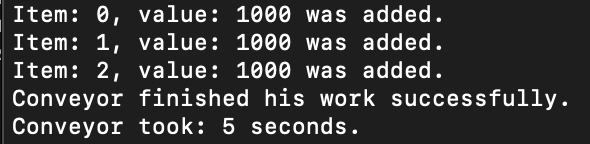
\includegraphics[scale=1]{Element3.png}}
\caption{Результат работы при 3 входных элементах}
\end{figure}

\begin{figure}[ht!]
\center{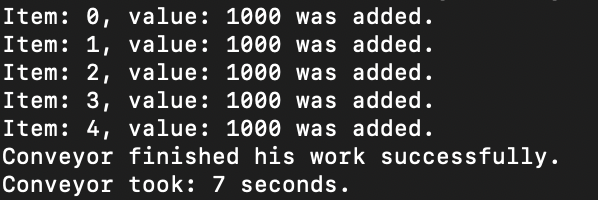
\includegraphics[scale=1]{Element5.png}}
\caption{Результат работы при 5 входных элементах}
\end{figure}

Как видно из приведенных результатов: один входной элемент, который должен быть обработан на всех трех лентах, обрабатывается последовательно и его суммарное время обработки равно 1 секунда * 3 ленты = 3 секунды. При этом уже для трех входных объектах суммарное время конвейерной обработки становится гораздо меньше суммарного времени последовательной обработки: 5 секунд < 9 секунд. Аналогичная ситуация наблюдается и для входной очереди из пяти элементов.

\section{Анализ лога}

\hspace{0.6cm}Для того, чтобы отследить работу потоков, необходимо получить лог-файл, отражающий время начала работы ленты над очередным заданием и время окончания этой работы. 
Например, на рисунке 4.4 представлен лог-файл для ситуации, когда генератор подал на вход конвейеру пять элементов.

\begin{figure}[ht!]
\center{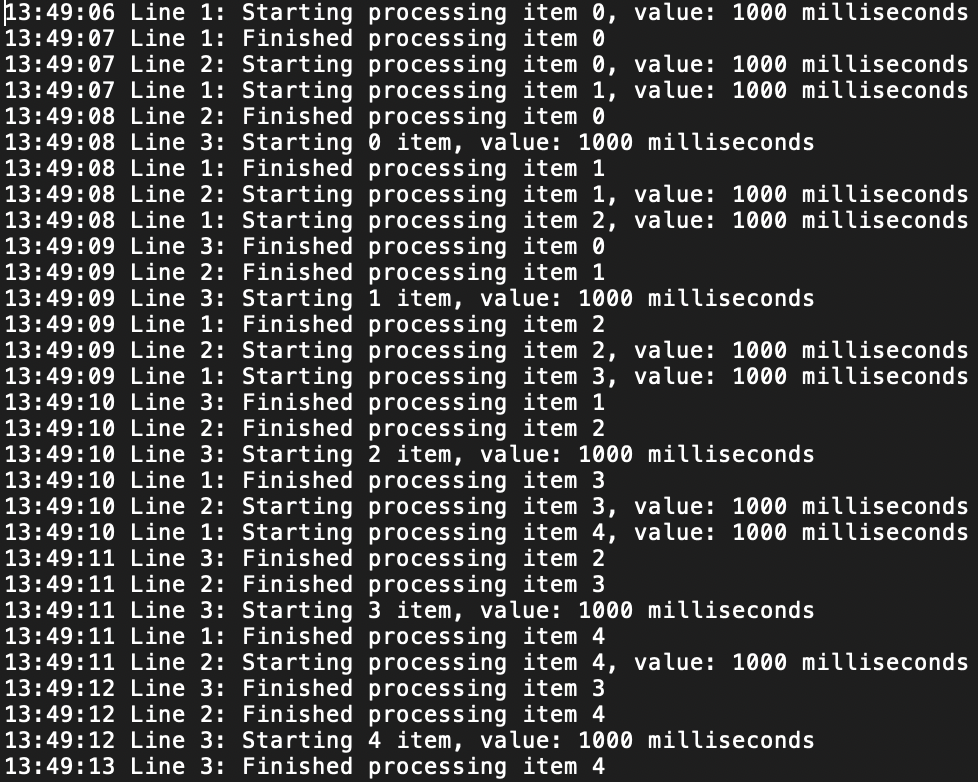
\includegraphics[scale=0.8]{Log5.png}}
\caption{Результирующий лог-файл при 5 входных элементах}
\end{figure}

\hspace{0.6cm}В первом столбце показано время записи, во втором лента конвейера, на которой производилась запись, далее указано начало или конец обработки и номер элемента, который обрабатывался. Если это начало обработки, то в конце указывается количество миллисекунд, которые должен обрабатываться этот элемент. Из представленного файла видно, что как только первый входной объект 0 item был обработан на первой ленте, его начинает обрабатывать вторая лента. В это время на первой ленте уже идет обработка следующего элемента. Как только на второй ленте закончилась обработка 0 item, начинает работать третья лента конвейера. 

Время обработки текущего элемента на всех трех лентах конвейера одинаковое,  поэтому ленты простаивают в течение работы программы, кроме ситуации в самом начале, когда первый элемент еще не поступил в очередь на обработку ко второй и третьей лентам. 

Рассмотрим другой пример, когда на вход подаются задачи, требующие на обработку одинакового количества времени, однако на второй ленте конвейера обработка будет занимать в 2 раза больше времени, чем на других лентах. На рисунке 4.5 представлен лог работы программы.

\begin{figure}[ht!]
\center{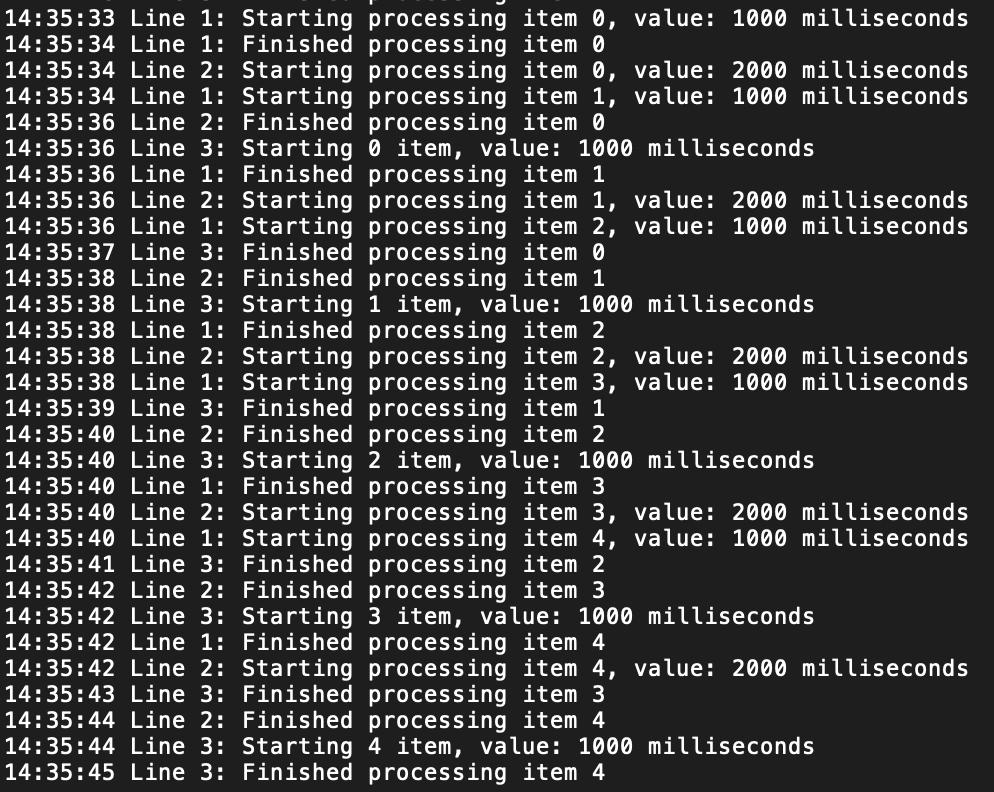
\includegraphics[scale=0.8]{LongLog.png}}
\caption{Результирующий лог-файл при увеличенном времени обработки на 2 ленте}
\end{figure}

Как видно из лог-файла, 3 лента конвейера простаивает 1 секунду на каждом элементе, кроме первого.

\section{Вывод}
\hspace{0.6cm} При анализе лога было выяснено, что при разном времени обработки на разных лентах, некоторые из них могут простаивать.

\newpage
\chapter*{Заключение}
\addcontentsline{toc}{chapter}{Заключение}
\hspace{0.6cm}В ходе лабораторной работы был изучен и реализован алгоритма, использующий конвейерную обработку данных с использованием методов распараллеливания процессов. Были выявлены оптимальные для конвейерной обработки параметры входных задач - сбалансированное время обработки данных на всех лентах конвейера.    
\end{document}